\section{Experiments}\label{sec:experiments}\label{sec:results}

This section reports the completed TE-Q-Transformer evaluation in five parts. Section~\ref{sec:experiment_setup} fixes the protocol, implementation, and comparison set. Section~\ref{sec:nasa_case} presents the primary NASA case study. Section~\ref{sec:calce} reports NASA$\rightarrow$CALCE zero-shot external validation. Section~\ref{sec:contemporary_comparison} compares the proposed model with the scored contemporary baselines. Section~\ref{sec:further_study} isolates physics-guided temperature encoding, the matched quantum representation, cell-wise generalization, and multi-seed variability. A held-out-temperature protocol was not executed; no unseen-temperature figure or table is included.

\subsection{Experiment Setup}
\label{sec:experiment_setup}

\subsubsection{Evaluation Protocol}
\label{sec:evaluation_protocol}

All NASA experiments use one fixed hybrid cross-cell split (Table~\ref{tab:exp_split}). Training uses B0005, B0006, B0007, B0029, B0030, B0031, and B0053 cycles 0--36 ($N=660$ discharge cycles). Testing uses B0018 ($n=132$), B0032 ($n=39$), and B0053 cycles 37--52 ($n=16$). B0018 and B0032 are unseen cells. B0053 cycles 37--52 are a temporal extrapolation on a cell that already contributed early cycles to training; B0053 is not an unseen cell. Nominal ($24\,^\circ$C), elevated ($43\,^\circ$C), and sub-ambient ($4\,^\circ$C) operating temperatures all appear in the training pool, so the NASA protocol is not an unseen-temperature experiment.

Cells and cycles are partitioned before windowing. Voltage, current, and normalized time are scaled with a min--max scaler fitted on the training partition only. Temperature remains in raw degrees Celsius. There is no independent test-cell normalization, no test-based hyperparameter search, no test-based checkpoint selection, and no test-set calibration. Reported NASA overall RMSE, MAE, MAPE, and $R^2$ are unweighted means of the three evaluation settings unless a table states otherwise.

CALCE CS2\_35--CS2\_38 is used only as zero-shot external cross-dataset / cross-laboratory validation of a frozen NASA checkpoint and the frozen NASA scaler. No CALCE cell is used for training, scaler fitting, or model selection. CALCE temperature is a constant $23\,^\circ$C ambient fill. This experiment is not evidence of unseen-temperature generalization.

\begin{table}[t]
\caption{Cross-cell data split and evaluation roles. B0053 is a temporal holdout, not an unseen cell.}\label{tab:exp_split}
\begin{tabular*}{\tblwidth}{@{}LLLL@{}}
\toprule
Dataset & Partition & Cells / cycles & Role \\
\midrule
NASA & Train & B0005, B0006, B0007, B0029, B0030, B0031, B0053 0--36 & Seen cells + early B0053 \\
NASA & Test & B0018 & Unseen cell, $24\,^\circ$C \\
NASA & Test & B0032 & Unseen cell, $43\,^\circ$C \\
NASA & Test & B0053 37--52 & Temporal extrapolation, $4\,^\circ$C \\
CALCE & Test only & CS2\_35, CS2\_36, CS2\_37, CS2\_38 & Zero-shot external cells, $23\,^\circ$C \\
\bottomrule
\end{tabular*}
\end{table}

\subsubsection{Implementation Details}
\label{sec:implementation_details}

Each input is a length-512 window with channels voltage, current, temperature ($^\circ$C), and intra-cycle normalized time. SOH is the cycle capacity divided by that cell's first-cycle capacity. Common optimization settings follow Table~\ref{tbl1}: AdamW with learning rate $10^{-3}$, batch size 8, maximum 80 epochs, gradient-norm clipping 1.0, and ReduceLROnPlateau (factor 0.5, patience 10). Early stopping uses training MSE with patience 20. No held-out validation split was used in the completed campaigns; the retained checkpoint is the lowest training-loss epoch. This is a protocol limitation and is not presented as a validation-based model-selection procedure.

The quantum circuit uses 4 qubits and is executed as a PennyLane \texttt{default.qubit} state-vector simulation, not on physical quantum hardware. Metrics are RMSE, MAE, MAPE (\%), $R^2$, and maximum absolute error (MaxE). E01--E06 use seed 42. E07 repeats the five designated models on seeds 42--46. Weight decay is $5\times10^{-2}$ in the E01/E04 reference training configuration and $1\times10^{-2}$ in the independent E06 retraining; those two TE-Q-Transformer numbers are therefore not interchangeable.

\subsubsection{Baseline and Comparison Methods}
\label{sec:baseline_comparison}

The scored E05 set comprises eight classical sequence models (LSTM, GRU, CNN1D, TCN, DLinear, Transformer, PatchTST, iTransformer), two hybrid quantum-recurrent models (QLSTM, QNN-GRU), and the proposed TE-Q-Transformer. Implementations follow official or paper-faithful sources where an official repository exists, with a shared seq-to-one NASA interface~\citep{wang2024state,zhang2023accurate,giuliano2025transformer,soon2025hybrid,wang2026prediction}. TimesNet was implemented and sanity-checked but excluded from the scored table because of disproportionate cost under the fixed $L=512$ protocol (approximately $14.3$ million parameters and about one hour per CPU epoch). A gate-level QGRU was implemented and sanity-checked; a completed scored NASA run is not present in the audited E05 metrics, so no QGRU test number is reported.

In E05 the ten baselines were trained from scratch on the NASA split. TE-Q-Transformer was held fixed at the previously validated E01/E04 checkpoint and was not retrained in E05. E06 retrains the five designated models independently. Parameter counts and E05 wall-clock times are listed in Table~\ref{tab:main_benchmark} and Table~\ref{tab:compute}.

\subsection{Case Study on the NASA Battery Dataset}
\label{sec:nasa_case}

\subsubsection{Dataset Description}
\label{sec:nasa_description}

The NASA Ames PCoE Li-ion ageing set~\cite{saha2007battery} is the primary benchmark. The archived data record voltage, current, and temperature during charge and discharge of commercial 18650 cells. Figure~\ref{fig:nasa_setup} summarizes the documented acquisition chain as a schematic; it is not a photograph of the NASA testbed. The cells used here span three ambient conditions: $24\,^\circ$C (B0005--B0007, B0018), $43\,^\circ$C (B0029--B0032), and $4\,^\circ$C (B0053). Cycle-level windows are linearly resampled to 512 points. The presence of all three temperatures in training means that strong NASA test scores do not establish unseen-temperature generalization.

\begin{figure}[t]
\centering
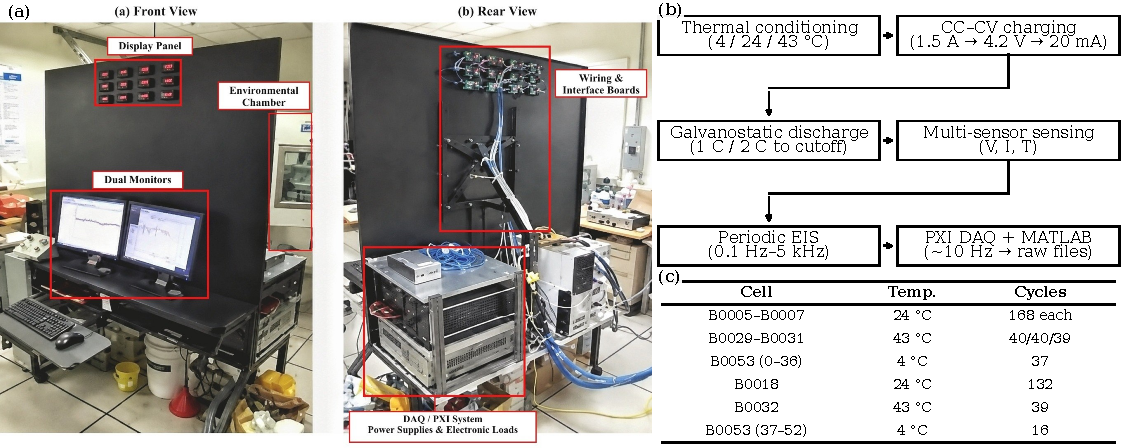
\includegraphics[width=\linewidth]{figs/fig2_nasa_experimental_setup.pdf}
\caption{NASA PCoE battery-data acquisition concept reconstructed from the official dataset description~\cite{saha2007battery}. This is an original schematic of the measurement chain, not a photograph of the physical apparatus.}
\label{fig:nasa_setup}
\end{figure}

\begin{table}[t]
\caption{NASA cycle counts used in the completed experiments.}\label{tab:nasa_stats}
\begin{tabular*}{\tblwidth}{@{}LLLL@{}}
\toprule
Cell & Ambient $T$ & Cycles used & Role \\
\midrule
B0005 / B0006 / B0007 & $24\,^\circ$C & $168$ each & Train \\
B0029 / B0030 & $43\,^\circ$C & $40$ each & Train \\
B0031 & $43\,^\circ$C & $39$ & Train \\
B0053 (0--36) & $4\,^\circ$C & $37$ & Train \\
B0018 & $24\,^\circ$C & $132$ & Unseen-cell test \\
B0032 & $43\,^\circ$C & $39$ & Unseen-cell test \\
B0053 (37--52) & $4\,^\circ$C & $16$ & Temporal test \\
\bottomrule
\end{tabular*}
\end{table}

\subsubsection{Evaluation Task Setup}
\label{sec:nasa_task_setup}

The NASA case study answers two complementary questions under one split. Unseen-cell generalization asks whether a model trained on B0005--B0007, B0029--B0031, and early B0053 can estimate SOH on B0018 and B0032. Temporal extrapolation asks whether the same model can continue the late-life segment of B0053 after seeing only cycles 0--36. The two settings are not equivalent: B0053 is partially observed, and the late tail contains only 16 cycles.

\subsubsection{Results and Analysis}
\label{sec:nasa_results}

E01 supplies the proposed-model reference (macro RMSE $0.0168$, MAE $0.0141$, $R^2$ $0.870$) that is reused as the frozen E05 TE-Q-Transformer entry. E02--E04 isolate temperature encoding and the matched quantum representation and are discussed in Section~\ref{sec:further_study}. E05 is the scored contemporary comparison on the same NASA split (Figure~\ref{fig:main_performance}; Table~\ref{tab:main_benchmark}).

Under the E05 protocol, TE-Q-Transformer recorded the lowest macro-averaged RMSE ($0.0168$), MAE ($0.0141$), and MAPE ($1.56\%$), and the highest macro-averaged $R^2$ ($0.870$), among the evaluated models. The closest scored baseline on RMSE was QNN-GRU ($0.0304$). The ranking is not uniform at the cell level. CNN1D recorded a lower RMSE on unseen B0018 ($0.0255$ versus $0.0271$), whereas TE-Q-Transformer recorded the lowest RMSE on unseen B0032 ($0.0119$) and on the B0053 temporal holdout ($0.0113$). iTransformer had the highest baseline $R^2$ ($0.533$). QLSTM did not improve on LSTM ($0.0445$ versus $0.0416$). These comparisons use a single seed and a NASA-only split; they are not a statistical test and not an unseen-temperature study.

E06 retrains five designated models and evaluates trajectory behaviour (Figure~\ref{fig:nasa_generalization}; Table~\ref{tab:e06_cells}). The E06 TE-Q-Transformer macro RMSE is $0.02387$, which differs from the frozen E05 reference ($0.01678$). The two numbers come from different trainings (E05 frozen E01/E04 checkpoint with weight decay $0.05$; E06 independent run with weight decay $0.01$) and are not substituted for one another. In the E06 five-model comparison, TE-Q-Transformer had the lowest RMSE on B0018 ($0.02758$), B0032 ($0.02036$), and B0053-test ($0.02366$). On B0032, PatchTST and iTransformer had lower MAE ($0.01714$ and $0.01850$ versus $0.01886$). The B0053-test $R^2$ of $0.184$ is limited by the short 16-cycle tail; RMSE and MAE are the more informative measures on that segment.

E07 then repeats those five models across five seeds (Section~\ref{sec:multiseed_analysis}). The NASA case study therefore supports a protocol-specific aggregate advantage for the frozen reference model in E05, a retained but numerically different E06 retraining result, and non-negligible seed variability in E07.

\begin{figure*}[t]
\centering
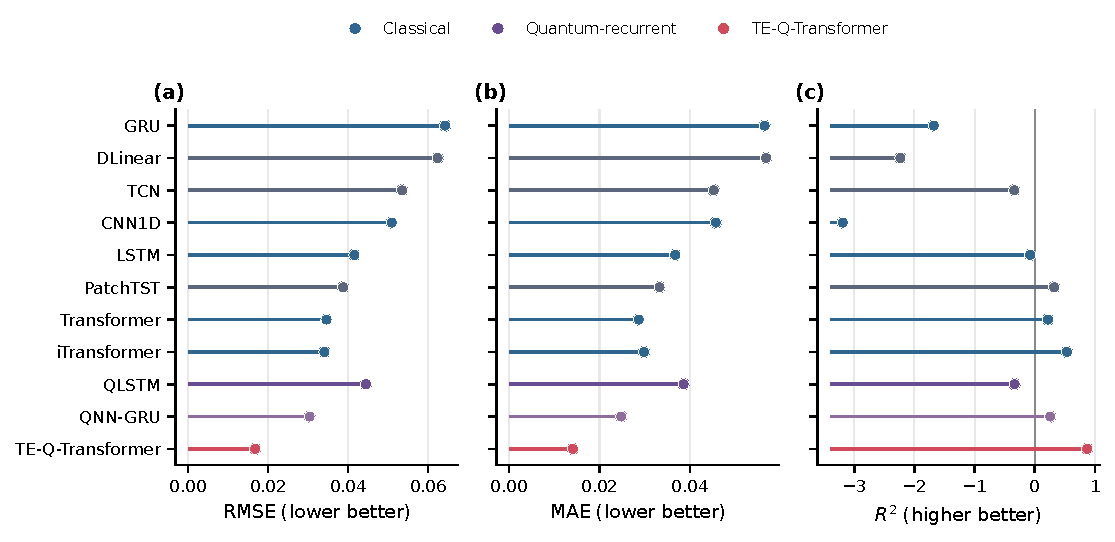
\includegraphics[width=\textwidth]{figs/fig6_main_performance.pdf}
\caption{E05 NASA macro-averaged performance for the ten scored baselines and the frozen TE-Q-Transformer reference. (a)~RMSE, (b)~MAE, (c)~$R^2$. Classical models are shown in blue/slate, quantum-recurrent baselines in purple, and TE-Q-Transformer in red. Single seed 42.}
\label{fig:main_performance}
\end{figure*}

\begin{figure*}[t]
\centering
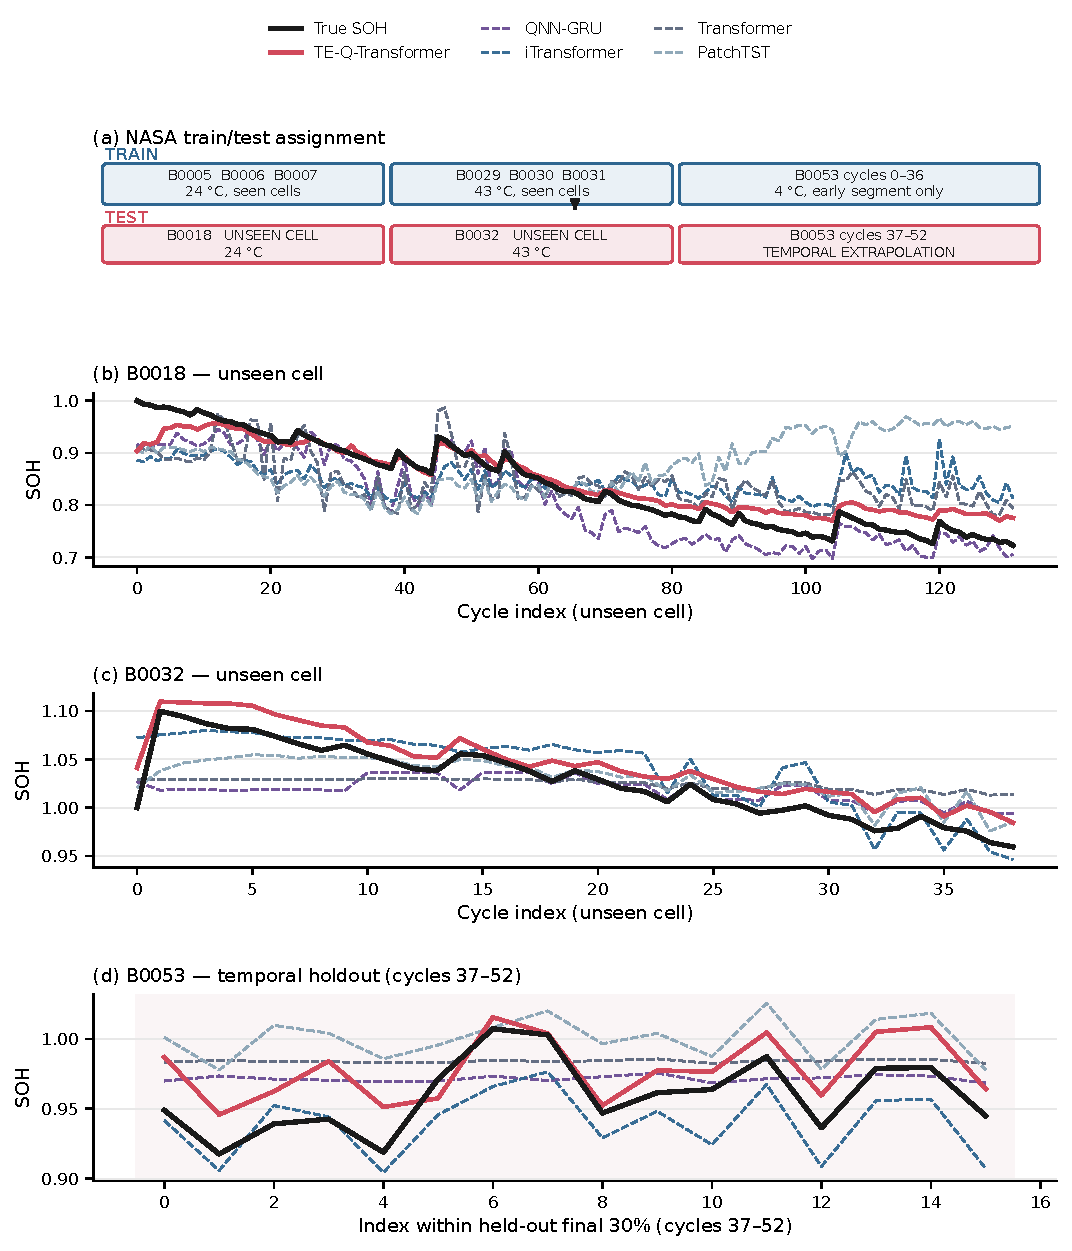
\includegraphics[width=\textwidth]{figs/fig9_nasa_generalization.pdf}
\caption{E06 predicted versus true SOH for the five designated models. (a)~B0018, unseen cell; (b)~B0032, unseen cell; (c)~B0053 cycles 37--52, temporal extrapolation. TE-Q-Transformer was retrained in E06 and is not the frozen E05 reference.}
\label{fig:nasa_generalization}
\end{figure*}

\subsection{External Validation on the CALCE Battery Dataset}
\label{sec:calce}

\subsubsection{Dataset Description}
\label{sec:calce_description}

CALCE CS2 cells from the University of Maryland~\citep{w9rg-7173-25} provide a second laboratory, chemistry, and cycling protocol. The CS2 series are prismatic lithium cobalt oxide cells (nominal $1.1$\,Ah) cycled with CCCV charge and $1$C discharge. Official Excel logs have no thermocouple column; temperature is filled at a constant $23\,^\circ$C ambient. The completed audit uses CS2\_35 ($n=880$), CS2\_36 ($n=968$), CS2\_37 ($n=1036$), and CS2\_38 ($n=1025$). Because ambient temperature is fixed, CALCE cannot support an unseen-temperature claim.

\subsubsection{Evaluation Protocol}
\label{sec:calce_protocol}

The audited CALCE experiment is zero-shot transfer of the frozen NASA TE-Q-Transformer checkpoint and the frozen NASA train-only scaler. All four CS2 cells are unseen external test cells. No CALCE-trained checkpoint, no CALCE scaler, and no CALCE hyperparameter search are used. This protocol is stricter than, and is not the same as, a CALCE-trained cross-cell split.

\subsubsection{Results and Analysis}
\label{sec:calce_results}

Table~\ref{tab:calce} and Figure~\ref{fig:calce_validation} report a negative transfer result. Pooled RMSE is $0.3325$, MAE $0.2676$, and $R^2$ $-1.789$ on $3909$ windows. Unweighted means over the four cells are RMSE $0.3302\pm0.0370$ and $R^2$ $-1.882\pm0.258$. Predictions remain near $1.01$ (documented range approximately $0.978$--$1.041$) while true SOH declines to about $0.14$. A constant predictor of $1.0$ has pooled RMSE $0.3277$, slightly lower than the frozen NASA model. Per-cycle prediction arrays were not archived; Figure~\ref{fig:calce_validation} therefore shows the audited true and predicted SOH ranges rather than reconstructed trajectories. The result is external cross-dataset evidence that the NASA-trained model does not track CALCE fade under zero-shot evaluation. It is not a CALCE-trained benchmark and not a temperature-generalization result.

\begin{table}[t]
\caption{NASA$\rightarrow$CALCE zero-shot results for the frozen TE-Q-Transformer. Lower RMSE/MAE and higher $R^2$ are better.}\label{tab:calce}
\begin{tabular*}{\tblwidth}{@{}LCCCC@{}}
\toprule
Cell & $n$ & RMSE~$\downarrow$ & MAE~$\downarrow$ & $R^2$~$\uparrow$ \\
\midrule
CS2\_35 & 880 & 0.2933 & 0.2415 & $-$2.070 \\
CS2\_36 & 968 & 0.3731 & 0.2937 & $-$1.567 \\
CS2\_37 & 1036 & 0.3483 & 0.2803 & $-$1.776 \\
CS2\_38 & 1025 & 0.3061 & 0.2524 & $-$2.115 \\
Pooled & 3909 & 0.3325 & 0.2676 & $-$1.789 \\
\bottomrule
\end{tabular*}
\end{table}

\begin{figure}[t]
\centering
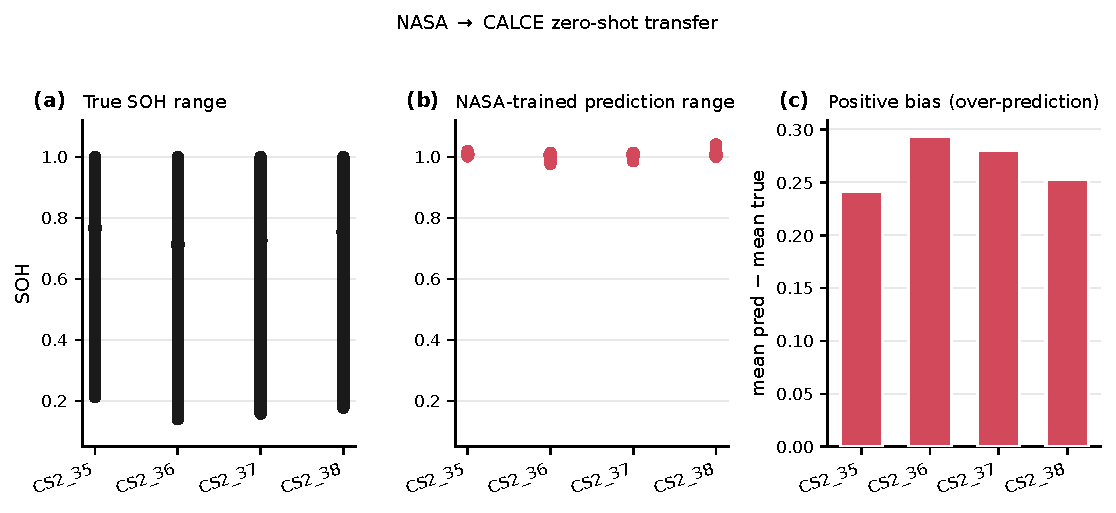
\includegraphics[width=\linewidth]{figs/fig12_calce_validation.pdf}
\caption{Audited NASA$\rightarrow$CALCE zero-shot ranges for (a)~CS2\_38 and (b)~CS2\_37. Black bars show the true SOH span; red bars show the frozen NASA prediction span. Per-cycle arrays were not archived.}
\label{fig:calce_validation}
\end{figure}

\subsection{Comparison with Contemporary Methods}
\label{sec:contemporary_comparison}

\subsubsection{Overall Benchmark Comparison}
\label{sec:overall_benchmark}

Table~\ref{tab:main_benchmark} lists the scored E05 metrics. TE-Q-Transformer achieved the lowest macro RMSE, MAE, and MAPE, and the highest macro $R^2$, among the evaluated models under the fixed NASA protocol. QNN-GRU is the nearest baseline on RMSE and MAE. Modern attention models (Transformer, PatchTST, iTransformer) occupy the next RMSE tier ($0.034$--$0.039$) with mixed $R^2$. Linear and convolutional baselines are weaker on the aggregate, and CNN1D and DLinear collapse on at least one evaluation setting (CNN1D $R^2=-10.45$ on B0053-test; DLinear $R^2=-7.16$ on B0032). The two quantum-recurrent models diverge: QNN-GRU is the strongest trained baseline, whereas QLSTM does not beat LSTM. E05 therefore does not support a generic quantum-module advantage. The contribution of the quantum embedding under matched physics is tested in E04, not in E05.

TE-Q MaxE in Table~\ref{tab:main_benchmark} is the true maximum absolute error on the $187$ test cycles ($0.1022$ on B0018). The stored reference CSV reports $0.0493$, which is the mean of the three cell-wise MaxE values and is not used here.

\begin{table*}[t]
\centering
\caption{E05 NASA main performance comparison. Overall metrics are unweighted means of B0018, B0032, and B0053-test. TE-Q-Transformer is the frozen E01/E04 reference (not retrained in E05). MaxE is the true maximum $|$error$|$. TimesNet and QGRU are not scored.}\label{tab:main_benchmark}
\footnotesize
\begin{tabular}{@{}lccccccc@{}}
\toprule
Model & RMSE~$\downarrow$ & MAE~$\downarrow$ & MAPE~$\downarrow$ & $R^2$~$\uparrow$ & MaxE~$\downarrow$ & Params & Train (s) \\
\midrule
LSTM & 0.0416 & 0.0367 & 4.07 & $-$0.076 & 0.0904 & 71\,105 & 24.5 \\
GRU & 0.0642 & 0.0565 & 6.22 & $-$1.680 & 0.1631 & 54\,465 & 22.3 \\
CNN1D & 0.0509 & 0.0457 & 4.78 & $-$3.191 & 0.1245 & 47\,041 & 25.1 \\
TCN & 0.0535 & 0.0452 & 5.09 & $-$0.341 & 0.1491 & 91\,841 & 34.0 \\
DLinear & 0.0624 & 0.0568 & 5.88 & $-$2.232 & 0.1853 & 1\,031 & 15.5 \\
Transformer & 0.0346 & 0.0287 & 3.14 & 0.218 & 0.1123 & 80\,257 & 61.6 \\
PatchTST & 0.0387 & 0.0333 & 3.69 & 0.321 & 0.1457 & 109\,962 & 63.1 \\
iTransformer & 0.0341 & 0.0298 & 3.28 & 0.533 & 0.1165 & 137\,473 & 58.7 \\
QLSTM & 0.0445 & 0.0386 & 4.35 & $-$0.336 & 0.1066 & 37\,853 & 282.3 \\
QNN-GRU & 0.0304 & 0.0248 & 2.61 & 0.258 & 0.0725 & 29\,533 & 284.8 \\
TE-Q-Transformer$^{\mathrm{a}}$ & \textbf{0.0168} & \textbf{0.0141} & \textbf{1.56} & \textbf{0.870} & 0.1022 & 92\,554 & --- \\
\bottomrule
\end{tabular}
\vspace{2pt}
\begin{minipage}{\textwidth}
\footnotesize $^{\mathrm{a}}$Frozen reference. E05 training time $18.5$\,s is not comparable to the ten trained baselines and is omitted. True MaxE $=0.1022$ (B0018).
\end{minipage}
\end{table*}

\subsubsection{Computational Analysis}
\label{sec:computational_analysis}

Table~\ref{tab:compute} reports parameter counts and recorded wall-clock times. TE-Q-Transformer has $92\,554$ trainable parameters, comparable to TCN ($91\,841$) and Transformer ($80\,257$), and larger than QNN-GRU ($29\,533$). It is not described as lightweight. E05 classical training times are $15$--$63$\,s; QLSTM and QNN-GRU require about $283$--$285$\,s on the simulator. Independent from-scratch TE-Q training in E06 required $564.7$\,s on CUDA. E04, which matches classical and quantum embeddings on CPU \texttt{default.qubit}, required $2179.9$\,s (classical + physics) versus $3599.3$\,s (quantum + physics). These times are simulated execution cost, not physical quantum-hardware cost, and do not support a computational quantum-advantage claim. The observed trade-off is higher simulation time for a lower NASA macro error in E04 and E05.

\begin{table}[t]
\caption{Computational record. E05 times are the ten trained baselines. E06 TE-Q time is an independent CUDA retraining. Quantum rows use a classical simulator.}\label{tab:compute}
\begin{tabular*}{\tblwidth}{@{}LCCC@{}}
\toprule
Model & Params & Train (s) & Infer. (s) \\
\midrule
DLinear & 1\,031 & 15.5 & 0.022 \\
QNN-GRU$^{\mathrm{s}}$ & 29\,533 & 284.8 & 0.342 \\
QLSTM$^{\mathrm{s}}$ & 37\,853 & 282.3 & 0.341 \\
CNN1D & 47\,041 & 25.1 & 0.043 \\
GRU & 54\,465 & 22.3 & 0.029 \\
LSTM & 71\,105 & 24.5 & 0.038 \\
Transformer & 80\,257 & 61.6 & 0.070 \\
TCN & 91\,841 & 34.0 & 0.057 \\
TE-Q-Transformer$^{\mathrm{s}}$ & 92\,554 & 564.7$^{\mathrm{b}}$ & 0.766$^{\mathrm{b}}$ \\
PatchTST & 109\,962 & 63.1 & 0.052 \\
iTransformer & 137\,473 & 58.7 & 0.045 \\
\bottomrule
\end{tabular*}
\vspace{2pt}
{\footnotesize $^{\mathrm{s}}$PennyLane \texttt{default.qubit} simulation. $^{\mathrm{b}}$E06 CUDA retraining, not the E05 frozen reference.}
\end{table}

\subsection{Further Study}
\label{sec:further_study}

\subsubsection{Physics-Guided Temperature Analysis}
\label{sec:physics_analysis}
\label{sec:ablation}

E02 asks whether replacing raw/min--max temperature with the Arrhenius gate reduces NASA error (Figure~\ref{fig:physics_contribution}a; Table~\ref{tab:physics}). Physics-guided encoding lowers macro RMSE from $0.0201$ to $0.0168$ ($16.5\%$ relative). The cell pattern is mixed: RMSE increases on unseen B0018 ($-17.5\%$) and decreases on B0032 ($+34.8\%$) and B0053-test ($+40.4\%$). The B0018 deterioration is retained in the figure; the macro gain is not uniform.

E03 then isolates the two kinetic terms (Figure~\ref{fig:physics_contribution}b). Combined SEI + plating has the lowest E03 macro RMSE ($0.0215$), versus plating-only $0.0249$ and SEI-only $0.0330$. On B0053-test, plating-only is best (RMSE $0.0171$ versus combined $0.0222$). E02 physics-guided and E03 combined are separate trainings and are not averaged.

Learned activation-energy parameters from the E03 checkpoints are reported in Table~\ref{tab:ea} as optimized model scalars (initialized at $3.0$, i.e.\ $30$\,kJ\,mol$^{-1}$ in the implementation scale). They are not independently measured physical constants.

\begin{table}[t]
\caption{Physics-guided temperature ablation (macro of B0018, B0032, B0053-test). E02 and E03 are separate campaigns.}\label{tab:physics}
\begin{tabular*}{\tblwidth}{@{}LCCCC@{}}
\toprule
Variant & RMSE & MAE & MAPE & $R^2$ \\
\midrule
E02 raw $T$ & 0.0201 & 0.0171 & 1.84 & 0.723 \\
E02 physics-guided $T$ & 0.0168 & 0.0141 & 1.56 & 0.870 \\
E03 SEI-only & 0.0330 & 0.0282 & 2.88 & 0.068 \\
E03 plating-only & 0.0249 & 0.0208 & 2.21 & 0.592 \\
E03 SEI + plating & 0.0215 & 0.0172 & 1.81 & 0.610 \\
\bottomrule
\end{tabular*}
\end{table}

\begin{table}[t]
\caption{Learned activation-energy parameters from E03 (seed 42). Values are implementation-scale scalars, not measured $E_a$.}\label{tab:ea}
\begin{tabular*}{\tblwidth}{@{}LCCC@{}}
\toprule
Variant & Init. & $E_{a,\mathrm{sei}}$ & $E_{a,\mathrm{pl}}$ \\
\midrule
SEI-only & 3.0 & 2.618 & --- \\
Plating-only & 3.0 & --- & 2.180 \\
SEI + plating & 3.0 & 1.981 & 2.820 \\
\bottomrule
\end{tabular*}
\end{table}

\begin{figure*}[t]
\centering
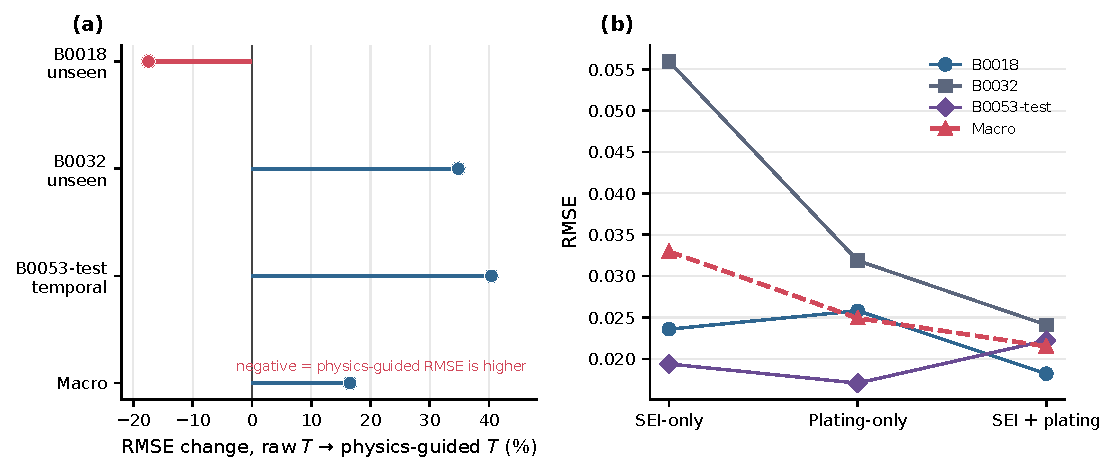
\includegraphics[width=\textwidth]{figs/fig7_physics_contribution.pdf}
\caption{Physics contribution. (a)~E02 percent RMSE change from raw temperature to physics-guided temperature; the B0018 bar is negative. (b)~E03 RMSE for SEI-only, plating-only, and combined pathways.}
\label{fig:physics_contribution}
\end{figure*}

\subsubsection{Quantum Representation Analysis}
\label{sec:quantum_analysis}

E04 holds the Arrhenius gate fixed and replaces the 4-qubit circuit with a capacity-matched classical MLP (Table~\ref{tab:e04}; Figure~\ref{fig:quantum_contribution}). Quantum + physics records macro RMSE $0.0215$ and $R^2$ $0.610$; classical + physics records $0.0431$ and $R^2$ $-0.746$. The quantum variant is better on all three NASA settings, including B0018. Parameter counts are nearly matched ($92\,554$ versus $92\,695$). Training on the CPU simulator is slower for the quantum model ($3599$\,s versus $2180$\,s). The result indicates additional predictive value of the simulated quantum representation under this matched protocol. It does not establish hardware speedup or a general quantum computational advantage.

\begin{table}[t]
\caption{E04 matched classical versus quantum representation (macro metrics).}\label{tab:e04}
\begin{tabular*}{\tblwidth}{@{}LCCCCC@{}}
\toprule
Variant & RMSE & MAE & $R^2$ & Params & Train (s) \\
\midrule
Classical + physics & 0.0431 & 0.0377 & $-$0.746 & 92\,695 & 2179.9 \\
Quantum + physics & 0.0215 & 0.0172 & 0.610 & 92\,554 & 3599.3 \\
\bottomrule
\end{tabular*}
\end{table}

\begin{figure}[t]
\centering
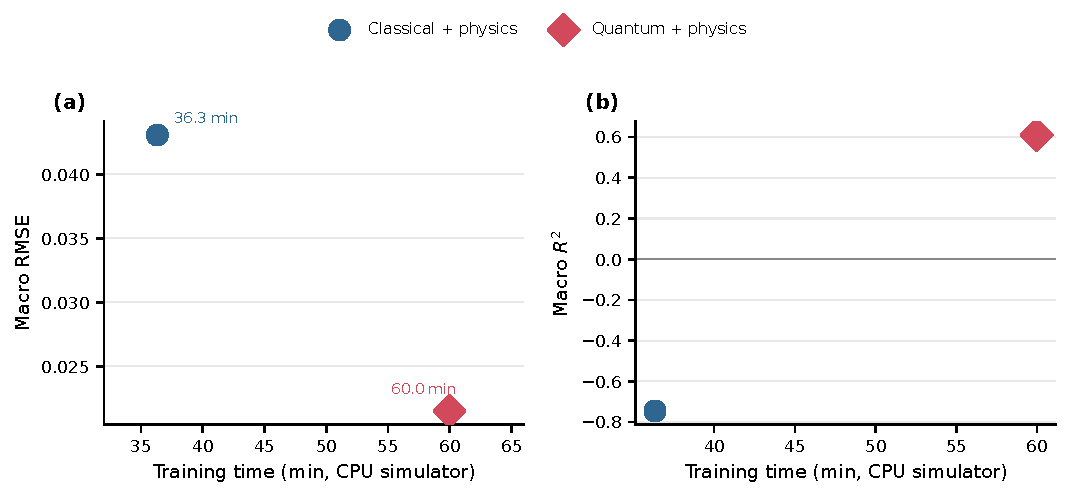
\includegraphics[width=\linewidth]{figs/fig8_quantum_contribution.pdf}
\caption{E04 accuracy--cost trade-off on the CPU PennyLane simulator. (a)~macro RMSE versus training time; (b)~macro $R^2$ versus training time.}
\label{fig:quantum_contribution}
\end{figure}

\subsubsection{Generalization Analysis}
\label{sec:generalization_analysis}

Table~\ref{tab:e06_cells} reports the E06 cell-wise scores. TE-Q-Transformer does not dominate every metric on every cell: PatchTST and iTransformer have lower MAE on unseen B0032, and several models remain close on the short B0053 tail. The unseen-cell mean RMSE for TE-Q-Transformer is $0.0240$ with a two-cell range of $0.0072$. QNN-GRU has a slightly smaller RMSE range ($0.0068$) at a higher mean ($0.0369$). These two-cell summaries describe observed variability only.

\begin{table*}[t]
\centering
\caption{E06 NASA cell-wise generalization for the five designated models. B0018/B0032 are unseen cells; B0053-test is temporal extrapolation.}\label{tab:e06_cells}
\footnotesize
\begin{tabular}{@{}lccccccccc@{}}
\toprule
 & \multicolumn{3}{c}{B0018 (unseen)} & \multicolumn{3}{c}{B0032 (unseen)} & \multicolumn{3}{c}{B0053-test (temporal)} \\
\cmidrule(lr){2-4}\cmidrule(lr){5-7}\cmidrule(lr){8-10}
Model & RMSE & MAE & $R^2$ & RMSE & MAE & $R^2$ & RMSE & MAE & $R^2$ \\
\midrule
TE-Q-Transformer & 0.0276 & 0.0215 & 0.890 & 0.0204 & 0.0189 & 0.713 & 0.0237 & 0.0209 & 0.184 \\
QNN-GRU & 0.0404 & 0.0344 & 0.765 & 0.0335 & 0.0248 & 0.221 & 0.0286 & 0.0241 & $-$0.195 \\
iTransformer & 0.0691 & 0.0624 & 0.311 & 0.0236 & 0.0185 & 0.613 & 0.0241 & 0.0214 & 0.154 \\
Transformer & 0.0604 & 0.0539 & 0.472 & 0.0335 & 0.0283 & 0.223 & 0.0358 & 0.0303 & $-$0.870 \\
PatchTST & 0.1249 & 0.1061 & $-$1.253 & 0.0222 & 0.0171 & 0.660 & 0.0449 & 0.0410 & $-$1.937 \\
\bottomrule
\end{tabular}
\end{table*}

\subsubsection{Multi-Seed Robustness}
\label{sec:multiseed_analysis}

E07 repeats the five E06 models on seeds 42--46 (Figure~\ref{fig:multiseed}; Table~\ref{tab:e07}). TE-Q-Transformer has the lowest mean RMSE ($0.0244\pm0.0096$) but a large coefficient of variation ($0.394$). Seed 43 is an adverse run (overall RMSE $0.0405$, B0032 $R^2=-2.13$). Seed 44 is the best TE-Q run (RMSE $0.0150$). QNN-GRU is more stable (RMSE $0.0381\pm0.0039$) at a higher mean error. Five predefined seeds do not constitute a statistical significance test, and the observed spread does not support a claim of uniform robustness.

\begin{table}[t]
\caption{E07 multi-seed robustness (mean $\pm$ SD over seeds 42--46). SD is the sample standard deviation, $n=5$.}\label{tab:e07}
\begin{tabular*}{\tblwidth}{@{}LCCC@{}}
\toprule
Model & RMSE & MAE & $R^2$ \\
\midrule
TE-Q-Transformer & $0.0244\pm0.0096$ & $0.0197\pm0.0084$ & $0.455\pm0.534$ \\
QNN-GRU & $0.0381\pm0.0039$ & $0.0328\pm0.0040$ & $-0.432\pm0.467$ \\
iTransformer & $0.0379\pm0.0112$ & $0.0327\pm0.0103$ & $0.133\pm0.733$ \\
Transformer & $0.0367\pm0.0071$ & $0.0312\pm0.0063$ & $0.167\pm0.298$ \\
PatchTST & $0.0466\pm0.0150$ & $0.0389\pm0.0126$ & $0.125\pm0.520$ \\
\bottomrule
\end{tabular*}
\end{table}

\begin{figure}[t]
\centering
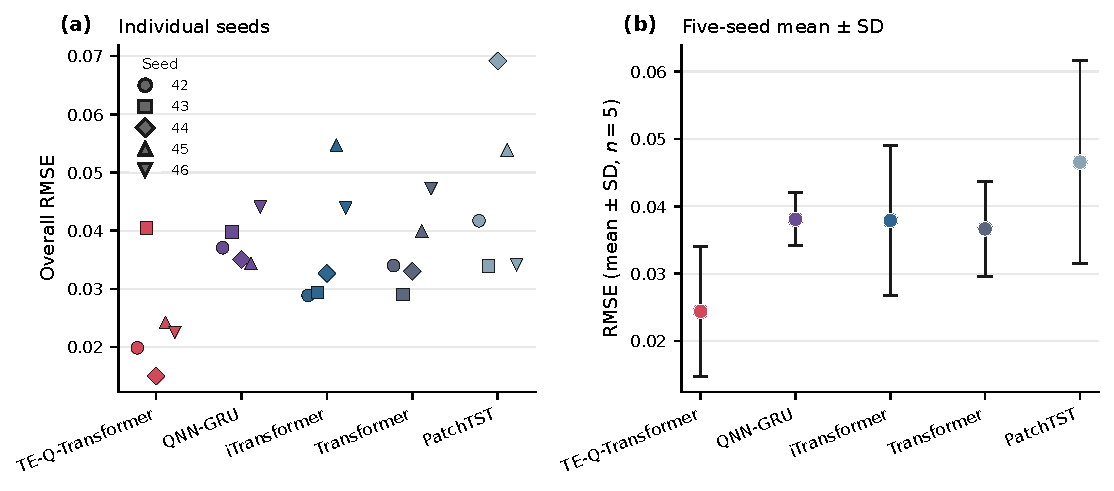
\includegraphics[width=\linewidth]{figs/fig11_multiseed_robustness.pdf}
\caption{E07 robustness. (a)~overall RMSE for each seed; (b)~mean $\pm$ SD over five seeds. TE-Q-Transformer seed 43 is the high-error red point.}
\label{fig:multiseed}
\end{figure}

\paragraph{Supplementary architectural ablation.}
Table~\ref{tab:s1_arch} retains the previously audited component ablation of the proposed architecture (rich entangler, temporal convolution, positional encoding, and CLS pooling). It is not an E02--E07 substitute and is not used to rank contemporary baselines.

\begin{table*}[t]
\centering
\small
\caption{Supplementary Table S1. Architectural component ablation on the NASA macro split (existing audited study). $\Delta$RMSE is relative to the full model.}\label{tab:s1_arch}\label{tab:nasa_ablation}
\begin{tabular}{@{}llcccccc@{}}
\toprule
Settings & Configuration & RMSE & MAE & MAPE & $R^2$ & MaxE & $\Delta$RMSE \\
\midrule
Basic entangler & Rich $\rightarrow$ basic & 0.0388 & 0.0320 & 3.53 & 0.342 & 0.0743 & $+0.0221$ \\
Pauli feature map & $+$ Pauli map & 0.0206 & 0.0166 & 1.78 & 0.774 & 0.0603 & $+0.0038$ \\
No temporal conv & $-$ temporal conv & 0.0261 & 0.0231 & 2.50 & 0.618 & 0.0554 & $+0.0093$ \\
GRU smoother & GRU replaces conv & 0.0274 & 0.0217 & 2.38 & 0.649 & 0.0610 & $+0.0107$ \\
No PE & $-$ positional encoding & 0.0330 & 0.0268 & 2.87 & 0.174 & 0.0862 & $+0.0162$ \\
Mean pooling & Mean pool, no CLS & 0.0237 & 0.0190 & 2.02 & 0.565 & 0.0642 & $+0.0069$ \\
Residual MLP & $+$ residual MLP & 0.0255 & 0.0214 & 2.29 & 0.545 & 0.0628 & $+0.0087$ \\
Full model & Rich, PE, conv $k{=}3$, CLS & 0.0168 & 0.0141 & 1.56 & 0.870 & 0.0493 & --- \\
\bottomrule
\end{tabular}
\end{table*}
